\item[(a)]
\section*{Exercise 2 Task (a): Visualizing the Spectrum of \(x(t)\)}

\subsection*{Objective}
This task aims to graphically demonstrate the real and imaginary parts of the spectrum \(X(f)\) of the signal \(x(t)\), based on the following refined definitions:

- Magnitude \(|X(f)|\):
  \[
  |X(f)| =
  \begin{cases}
  A & \text{for } -5 \leq f \leq -1 \text{ and } 1 \leq f \leq 5 \\
  -Af & \text{for } -1 < f < 0 \\
  Af & \text{for } 0 \leq f < 1 \\
  A & \text{at } f = -1, 1 \\
  0 & \text{otherwise}
  \end{cases}
  \]

- Phase \(\phi_x(f)\):
  \[
  \phi_x(f) =
  \begin{cases}
  \frac{\pi}{2} & \text{if } f < 0 \\
  -\frac{\pi}{2} & \text{if } f > 0 \\
  0 & \text{if } f = 0 \text{ or } |f| > 5
  \end{cases}
  \]

\subsection*{Analysis}
Detailed visual analysis is conducted through plots that clearly depict the real and imaginary components of the spectrum.
These plots in Figure~\ref{fig:spectrum_analysis_a} validate our theoretical understanding and provide a clear, visual confirmation of the spectrum's behavior.

\begin{figure}[h]
    \centering
    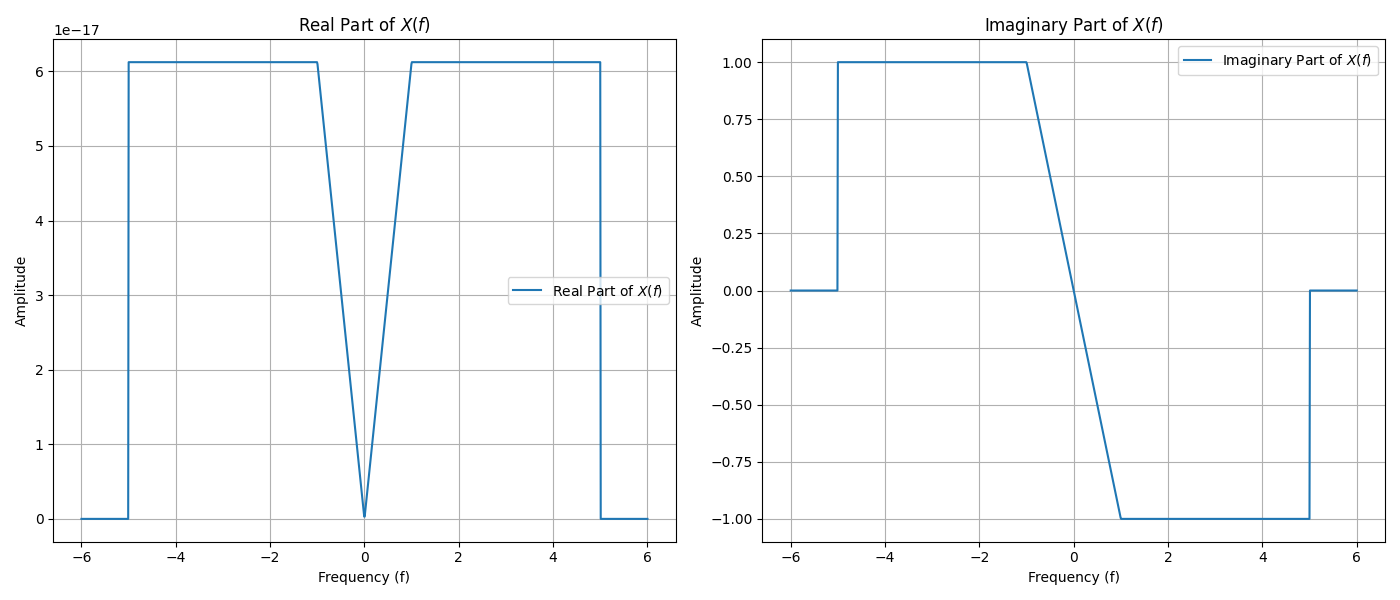
\includegraphics[width=0.9\textwidth]{fig/ex2_task_a_spectrum_analysis}
    \caption{Real and Imaginary parts of the spectrum \(X(f)\)}
    \label{fig:spectrum_analysis_a}
\end{figure}

\subsection*{Conclusion}
The spectral analysis demonstrates the direct impact of the magnitude and phase definitions on the signal's frequency domain behavior.